% !TeX program = xelatex
\documentclass[aspectratio=169,10pt]{beamer}

\usetheme{default}
\usefonttheme[onlymath]{serif}

\usepackage{amsmath}
\usepackage{amssymb}
\usepackage{array}
\usepackage{booktabs}
\usepackage{graphicx}
\usepackage{tabularx}
\usepackage{tikz}
\usepackage{iftex}
\usetikzlibrary{positioning,arrows.meta}

\ifPDFTeX
  \usepackage[utf8]{inputenc}
  \usepackage[T1]{fontenc}
  \usepackage{CJKutf8}
  \AtBeginDocument{\begin{CJK*}{UTF8}{gbsn}}
  \AtEndDocument{\end{CJK*}}
\else
  \usepackage{fontspec}
  \usepackage{xeCJK}
  \IfFontExistsTF{Times New Roman}{\setmainfont{Times New Roman}}{\setmainfont{TeX Gyre Termes}}
  \IfFontExistsTF{Arial}{\setsansfont{Arial}}{\setsansfont{TeX Gyre Heros}}
  \IfFontExistsTF{STSong}{%
    \setCJKmainfont{STSong}%
  }{%
    \IfFontExistsTF{FandolSong-Regular}{\setCJKmainfont{FandolSong-Regular}}{\setCJKmainfont{Noto Serif CJK SC}}%
  }
  \IfFontExistsTF{PingFang SC}{%
    \setCJKsansfont{PingFang SC}%
  }{%
    \IfFontExistsTF{FandolHei-Regular}{\setCJKsansfont{FandolHei-Regular}}{\setCJKsansfont{Noto Sans CJK SC}}%
  }
\fi
\renewcommand{\familydefault}{\sfdefault}
\graphicspath{{figs/}}

\definecolor{BrandOrange}{RGB}{243,93,0}
\definecolor{BrandOrangeDark}{RGB}{184,67,0}
\definecolor{BrandOrangeLight}{RGB}{255,239,232}
\definecolor{BrandGray}{RGB}{92,92,92}
\definecolor{BrandInk}{RGB}{34,34,34}
\definecolor{BrandBlue}{RGB}{32,88,148}

\setbeamertemplate{navigation symbols}{}
\setbeamertemplate{blocks}[rounded]
\setbeamertemplate{itemize item}{\color{BrandOrange}$\blacktriangleright$}
\setbeamertemplate{itemize subitem}{\color{BrandOrange}$\bullet$}
\setbeamercolor{normal text}{fg=BrandInk,bg=white}
\setbeamercolor{structure}{fg=BrandOrange}
\setbeamercolor{block title}{fg=white,bg=BrandOrange}
\setbeamercolor{block body}{fg=BrandInk,bg=BrandOrangeLight}
\setbeamercolor{alerted text}{fg=BrandOrangeDark}

\setlength{\parskip}{0.2em}
\setlength{\tabcolsep}{4pt}
\renewcommand{\arraystretch}{1.18}

\newcommand{\mgray}[1]{\textcolor{BrandGray}{#1}}
\newcommand{\mred}[1]{\textcolor{BrandOrangeDark}{#1}}
\newcommand{\source}[1]{\vspace{0.12em}{\tiny\color{BrandGray}Source: #1\par}}
\newcommand{\tightitems}{\setlength{\itemsep}{0.35em}}

\newcommand{\contentheader}[1]{%
  \vspace*{0.05em}%
  {\noindent\color{BrandOrange}\rule{0.42em}{0.42em}\hspace{0.50em}\bfseries\Large #1\par}%
  \vspace{0.15em}%
  {\color{BrandOrange}\rule{\textwidth}{1.4pt}\par}%
  \vspace{0.42em}%
}

\newcommand{\titleslide}{%
  \begin{tikzpicture}[remember picture,overlay]
    \fill[BrandOrange] (current page.south west) rectangle (current page.north east);
    \node[align=center,text=white,font=\bfseries\fontsize{22}{26}\selectfont] at ([yshift=0.65cm]current page.center) {Deep Limit Order Book Forecasting};
    \node[align=center,text=white,font=\Large] at ([yshift=-0.22cm]current page.center) {A Microstructure-First Introduction};
    \node[align=center,text=white,font=\normalsize] at ([yshift=-1.45cm]current page.center) {Yida Ding \quad \today};
  \end{tikzpicture}
}

\title{Deep Limit Order Book Forecasting}
\subtitle{A Microstructure-First Introduction}
\author{Yida Ding}
\date{\today}

\begin{document}
\small

\section{Cover}
\begin{frame}[plain]
\titleslide
\end{frame}

\section{Roadmap}
\begin{frame}[plain]
\contentheader{Opening Questions}
\begin{columns}[T,totalwidth=\textwidth]
\begin{column}{0.48\textwidth}
\begin{block}{Keep these in mind}
\begin{itemize}\tightitems
  \item What exactly is a LOB forecasting model predicting?
  \item Why do tick size, spread, and horizon change the difficulty?
  \item Why can a classifier be accurate but still be weak as a trading signal?
\end{itemize}
\end{block}
\end{column}
\begin{column}{0.48\textwidth}
\centering
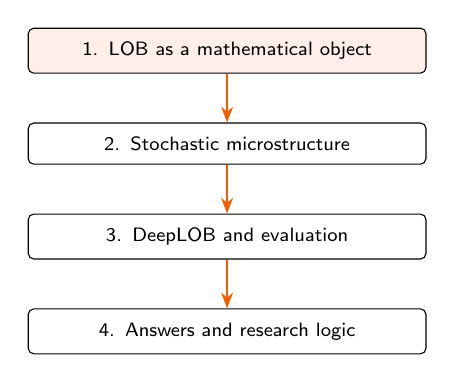
\begin{tikzpicture}[node distance=0.62cm,every node/.style={font=\scriptsize}]
\node[draw,rounded corners=2pt,fill=BrandOrangeLight,text width=4.7cm,align=center,inner sep=5pt] (a) {1. LOB as a mathematical object};
\node[draw,rounded corners=2pt,fill=white,text width=4.7cm,align=center,inner sep=5pt,below=of a] (b) {2. Stochastic microstructure};
\node[draw,rounded corners=2pt,fill=white,text width=4.7cm,align=center,inner sep=5pt,below=of b] (c) {3. DeepLOB and evaluation};
\node[draw,rounded corners=2pt,fill=white,text width=4.7cm,align=center,inner sep=5pt,below=of c] (d) {4. Answers and research logic};
\draw[-{Stealth[length=2mm]},BrandOrange,thick] (a) -- (b);
\draw[-{Stealth[length=2mm]},BrandOrange,thick] (b) -- (c);
\draw[-{Stealth[length=2mm]},BrandOrange,thick] (c) -- (d);
\end{tikzpicture}
\end{column}
\end{columns}
\end{frame}

\begin{frame}[plain]
\contentheader{Papers and Roles}
\scriptsize
\begin{tabularx}{\textwidth}{>{\raggedright\arraybackslash}p{3.1cm}X>{\raggedright\arraybackslash}p{4.0cm}}
\toprule
Paper & Role & How we use it \\
\midrule
Microstructural Guide & Main paper: explains LOB predictability through market structure & Labels, tick regimes, MCC, and \(p_T\) \\
DeepLOB & Canonical baseline: treats the LOB as a structured time series & Model principle, not engineering details \\
Ait-Sahalia et al. & Shows short-lived high-frequency predictability & Why horizon and latency matter \\
HLOB & Encodes structural dependence inside the book & Example of a stronger inductive bias \\
Benchmark Study & Shows single-dataset scores are fragile & Generalization warning \\
\bottomrule
\end{tabularx}
\end{frame}

\section{LOB Basics}
\begin{frame}[plain]
\contentheader{LOB 是什么：一个状态快照}
\begin{columns}[T,totalwidth=\textwidth]
\begin{column}{0.52\textwidth}
\begin{itemize}\tightitems
  \item LOB 记录还没有成交的买单和卖单。
  \item 每一档有价格和数量：卖一、卖二、买一、买二等。
  \item 深度学习常用前 \(L=10\) 档，把一个快照写成向量。
\end{itemize}
\vspace{0.3em}
\begin{block}{一条 LOB 记录}
\[
L(\tau)=
\{p^{ask}_{\ell},v^{ask}_{\ell},p^{bid}_{\ell},v^{bid}_{\ell}\}_{\ell=1}^{L}
\in\mathbb{R}^{4L}.
\]
\end{block}
\end{column}
\begin{column}{0.44\textwidth}
\begin{block}{模型看到的输入}
\[
X_\tau =
\big(L(\tau-T+1),\ldots,L(\tau)\big)
\]
\[
X_\tau\in\mathbb{R}^{T\times4L}
\]
\end{block}
\begin{block}{直觉}
不是一根价格线，而是一段“买卖盘形状”的电影。
\end{block}
\end{column}
\end{columns}
\end{frame}

\begin{frame}[plain]
\contentheader{Microstructure Model: A Jump Process}
\begin{columns}[T,totalwidth=\textwidth]
\begin{column}{0.50\textwidth}
\begin{itemize}\tightitems
  \item A useful abstraction is a continuous-time state process:
  \[
    Q_t=(Q_t^{b,1},\ldots,Q_t^{b,L},Q_t^{a,1},\ldots,Q_t^{a,L}).
  \]
  \item Each coordinate is queue size at one bid/ask level.
  \item Limit orders, market orders, and cancellations are jumps of \(Q_t\).
\end{itemize}
\end{column}
\begin{column}{0.46\textwidth}
\begin{block}{Point-process view}
\[
dQ_t=\sum_{e\in\mathcal{E}} \nu_e(Q_{t-})\,dN_t^e
\]
\[
\mathbb{P}(dN_t^e=1\mid\mathcal{F}_{t-})
\approx \lambda_e(Q_{t-})\,dt
\]
\end{block}
\begin{block}{Intuition}
The book is not a smooth curve; it is a queueing system hit by random order-flow events.
\end{block}
\end{column}
\end{columns}
\source{Cont and de Larrard (2013); Abergel and Jedidi (2013).}
\end{frame}

\begin{frame}[plain]
\contentheader{Why This Model Explains Predictability}
\begin{columns}[T,totalwidth=\textwidth]
\begin{column}{0.48\textwidth}
\begin{block}{Price moves when a queue is depleted}
\scriptsize
\[
\tau_a=\inf\{t:Q_t^{a,1}=0\}
\]
\[
\tau_b=\inf\{t:Q_t^{b,1}=0\}
\]
\[
\text{next move}=
\begin{cases}
\text{up}, & \tau_a<\tau_b,\\
\text{down}, & \tau_b<\tau_a.
\end{cases}
\]
\end{block}
\end{column}
\begin{column}{0.48\textwidth}
\begin{itemize}\tightitems
  \item Queue imbalance is predictive because it changes depletion probabilities.
  \[
    I_t=\frac{Q_t^{b,1}-Q_t^{a,1}}{Q_t^{b,1}+Q_t^{a,1}}.
  \]
  \item Event clustering matters: order arrivals are often self- and cross-exciting.
  \[
    \lambda_i(t)=\mu_i+\sum_j\int_0^t \phi_{ij}(t-s)\,dN_j(s).
  \]
  \item Deep models are useful because they learn nonlinear approximations to these conditional probabilities.
\end{itemize}
\end{column}
\end{columns}
\source{Cont and de Larrard (2013); Bacry, Mastromatteo and Muzy (2015).}
\end{frame}

\begin{frame}[plain]
\contentheader{预测目标：未来中间价方向}
\begin{columns}[T,totalwidth=\textwidth]
\begin{column}{0.48\textwidth}
\begin{block}{中间价与价差}
\[
m_\tau=\frac{p^{ask}_{1}(\tau)+p^{bid}_{1}(\tau)}{2}
\]
\[
\sigma_\tau=p^{ask}_{1}(\tau)-p^{bid}_{1}(\tau)
\]
\end{block}
\begin{itemize}\tightitems
  \item \(m_\tau\)：常用来定义方向。
  \item \(\sigma_\tau\)：买卖价差，也是交易摩擦。
\end{itemize}
\end{column}
\begin{column}{0.48\textwidth}
\begin{block}{三分类标签}
\[
y_\tau =
\begin{cases}
-1, & m_{\tau+\Delta\tau}-m_\tau\le -\theta,\\
0, & |m_{\tau+\Delta\tau}-m_\tau|<\theta,\\
+1, & m_{\tau+\Delta\tau}-m_\tau\ge +\theta.
\end{cases}
\]
\end{block}
\begin{itemize}\tightitems
  \item \(\theta\)：tick size，最小价格变动单位。
  \item \(\Delta\tau\)：未来多少次 LOB 更新，而不是固定秒数。
\end{itemize}
\end{column}
\end{columns}
\end{frame}

\section{Main Paper}
\begin{frame}[plain]
\contentheader{主论文到底研究什么}
\begin{columns}[T,totalwidth=\textwidth]
\begin{column}{0.48\textwidth}
\begin{block}{实验设置}
\begin{itemize}\tightitems
  \item 15 只 NASDAQ 股票，2017--2019 年。
  \item LOBSTER 逐笔订单簿数据。
  \item 输入：最近 100 次 LOB 更新，前 10 档。
  \item 输出：\(H_{10},H_{50},H_{100}\) 后的方向。
\end{itemize}
\end{block}
\end{column}
\begin{column}{0.48\textwidth}
\begin{block}{真正的问题}
\begin{itemize}\tightitems
  \item 不只是“DeepLOB 分数多少”。
  \item 而是：哪些股票更容易预测？为什么？
  \item 分类指标好，是否意味着信号可以形成完整交易？
\end{itemize}
\end{block}
\end{column}
\end{columns}
\vspace{0.35em}
\centering
\begin{tikzpicture}[node distance=0.65cm,every node/.style={font=\scriptsize}]
\node[draw,rounded corners=2pt,fill=BrandOrangeLight,inner sep=5pt] (a) {LOB 数据};
\node[draw,rounded corners=2pt,fill=white,inner sep=5pt,right=of a] (b) {微观结构分组};
\node[draw,rounded corners=2pt,fill=white,inner sep=5pt,right=of b] (c) {DeepLOB 预测};
\node[draw,rounded corners=2pt,fill=white,inner sep=5pt,right=of c] (d) {MCC + \(p_T\)};
\draw[-{Stealth[length=2mm]},BrandOrange,thick] (a) -- (b);
\draw[-{Stealth[length=2mm]},BrandOrange,thick] (b) -- (c);
\draw[-{Stealth[length=2mm]},BrandOrange,thick] (c) -- (d);
\end{tikzpicture}
\end{frame}

\begin{frame}[plain]
\contentheader{LOBFrame：把流程标准化}
\centering
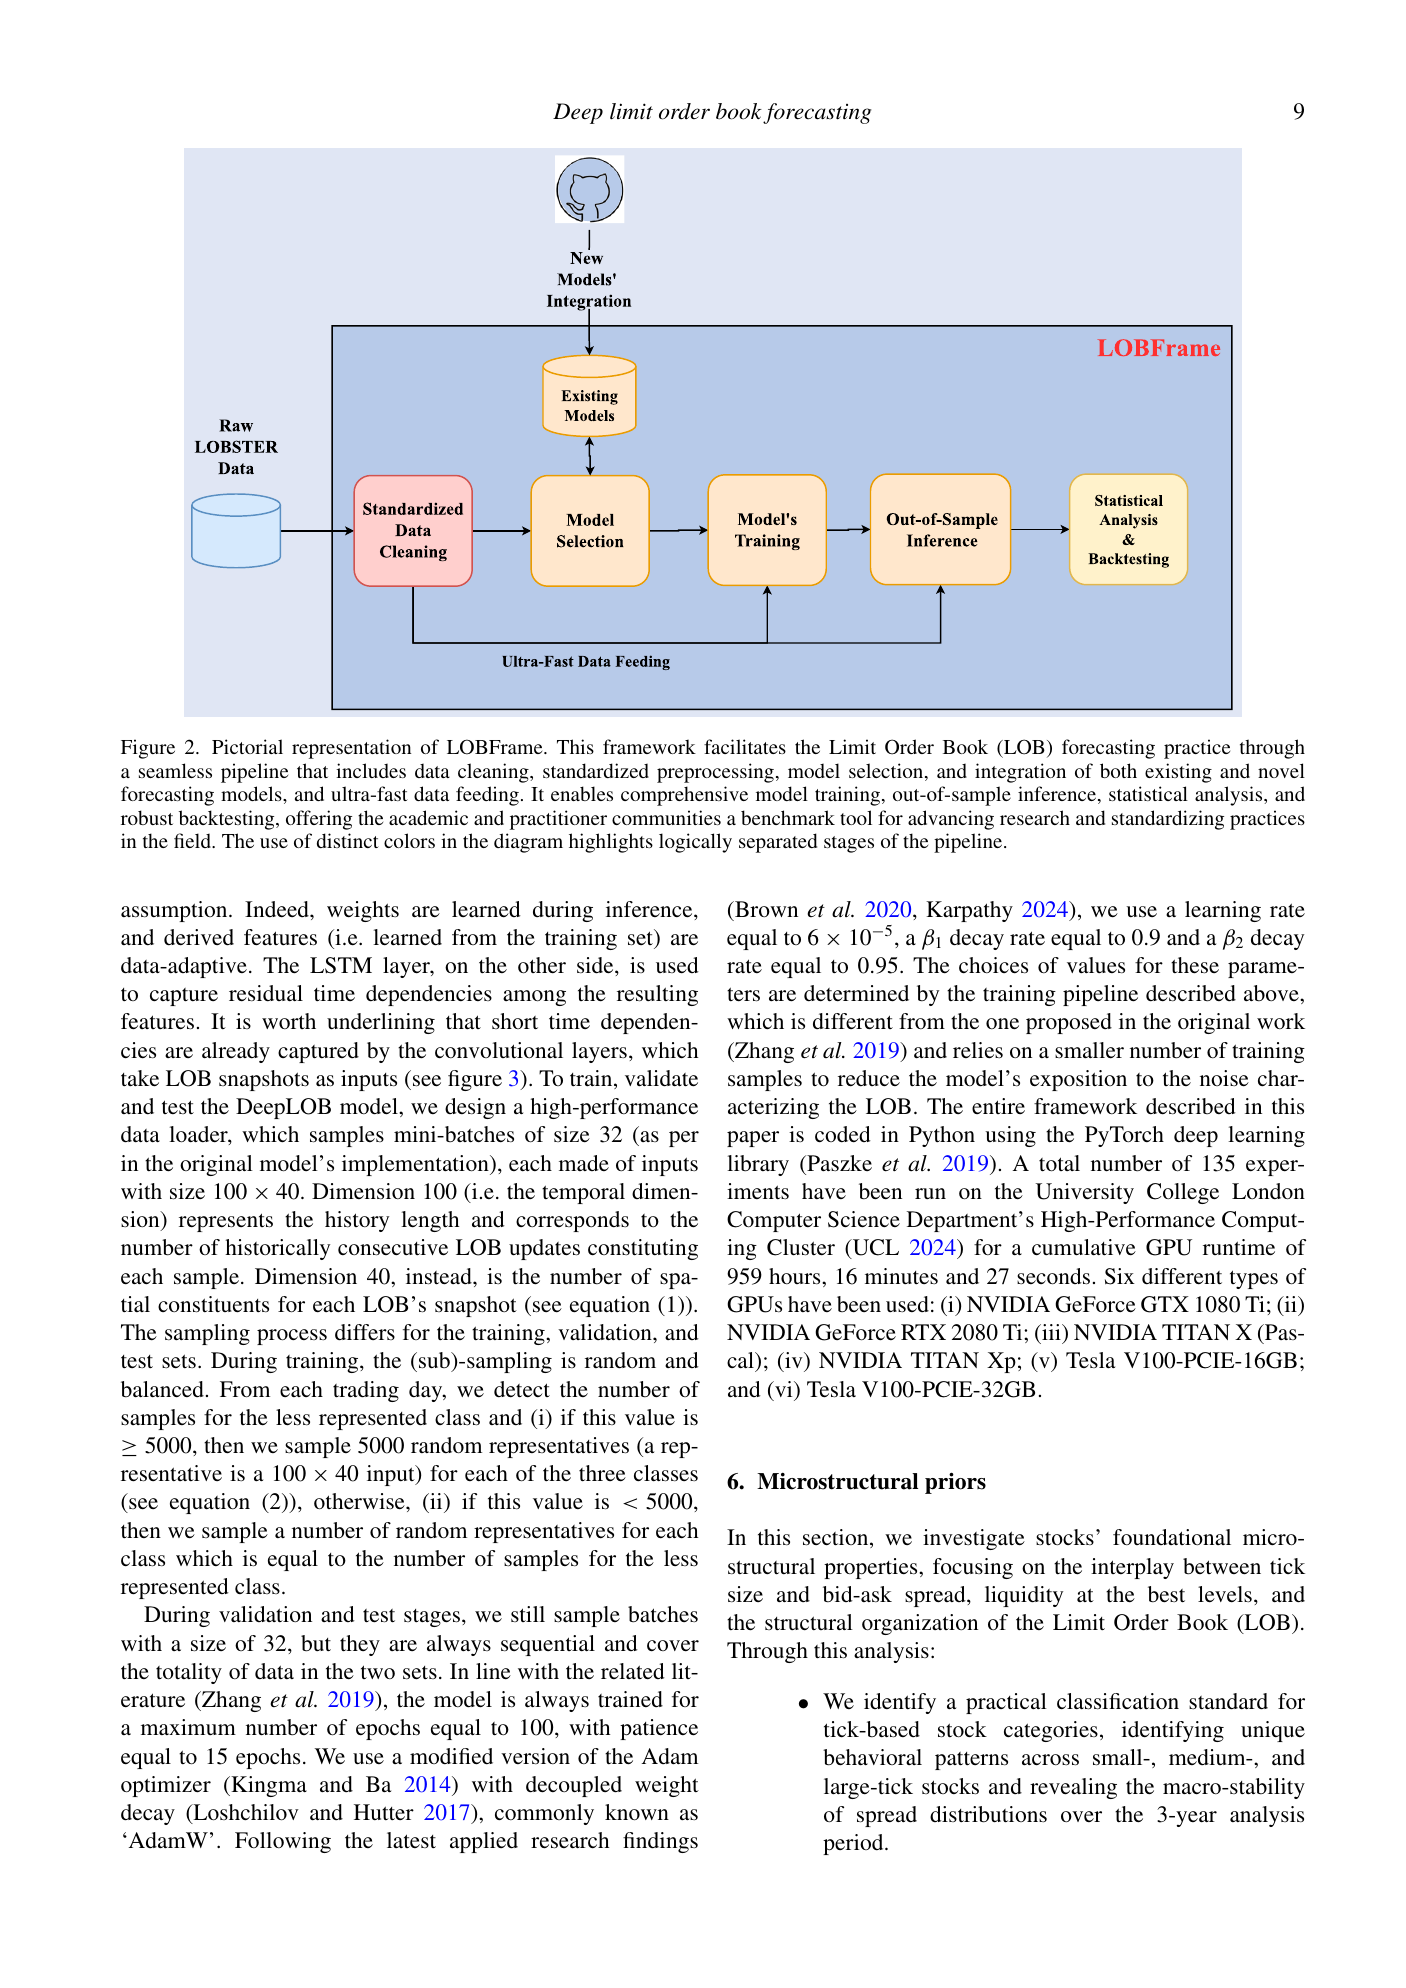
\includegraphics[width=0.96\textwidth,height=0.72\textheight,keepaspectratio]{lobframe_fig2.png}
\source{Briola et al., ``Deep Limit Order Book Forecasting: A Microstructural Guide'', Figure 2.}
\end{frame}

\begin{frame}[plain]
\contentheader{Tick size：这篇文章的核心变量}
\begin{columns}[T,totalwidth=\textwidth]
\begin{column}{0.50\textwidth}
\begin{block}{按价差相对 tick 分类}
\[
\bar{\sigma}=\mathbb{E}[\sigma_\tau],
\qquad r=\frac{\bar{\sigma}}{\theta}
\]
\[
\begin{array}{ll}
\text{small-tick}  & \bar{\sigma}>3\theta,\\
\text{medium-tick} & 1.5\theta<\bar{\sigma}<3\theta,\\
\text{large-tick}  & \bar{\sigma}<1.5\theta.
\end{array}
\]
\end{block}
\end{column}
\begin{column}{0.46\textwidth}
\begin{itemize}\tightitems
  \item large-tick：价差常接近 1 tick，最优档队列很重要。
  \item small-tick：价差可以展开成很多 tick，结构更稀疏、更不稳定。
  \item 因此，同样的标签规则，在不同股票上不是同一个难度。
\end{itemize}
\vspace{0.25em}
\begin{block}{初学者理解}
tick size 不只是交易所规则；它决定“价格动一下”在这个市场里有多大意义。
\end{block}
\end{column}
\end{columns}
\end{frame}

\begin{frame}[plain]
\contentheader{DeepLOB：模型只讲思路}
\begin{columns}[T,totalwidth=\textwidth]
\begin{column}{0.52\textwidth}
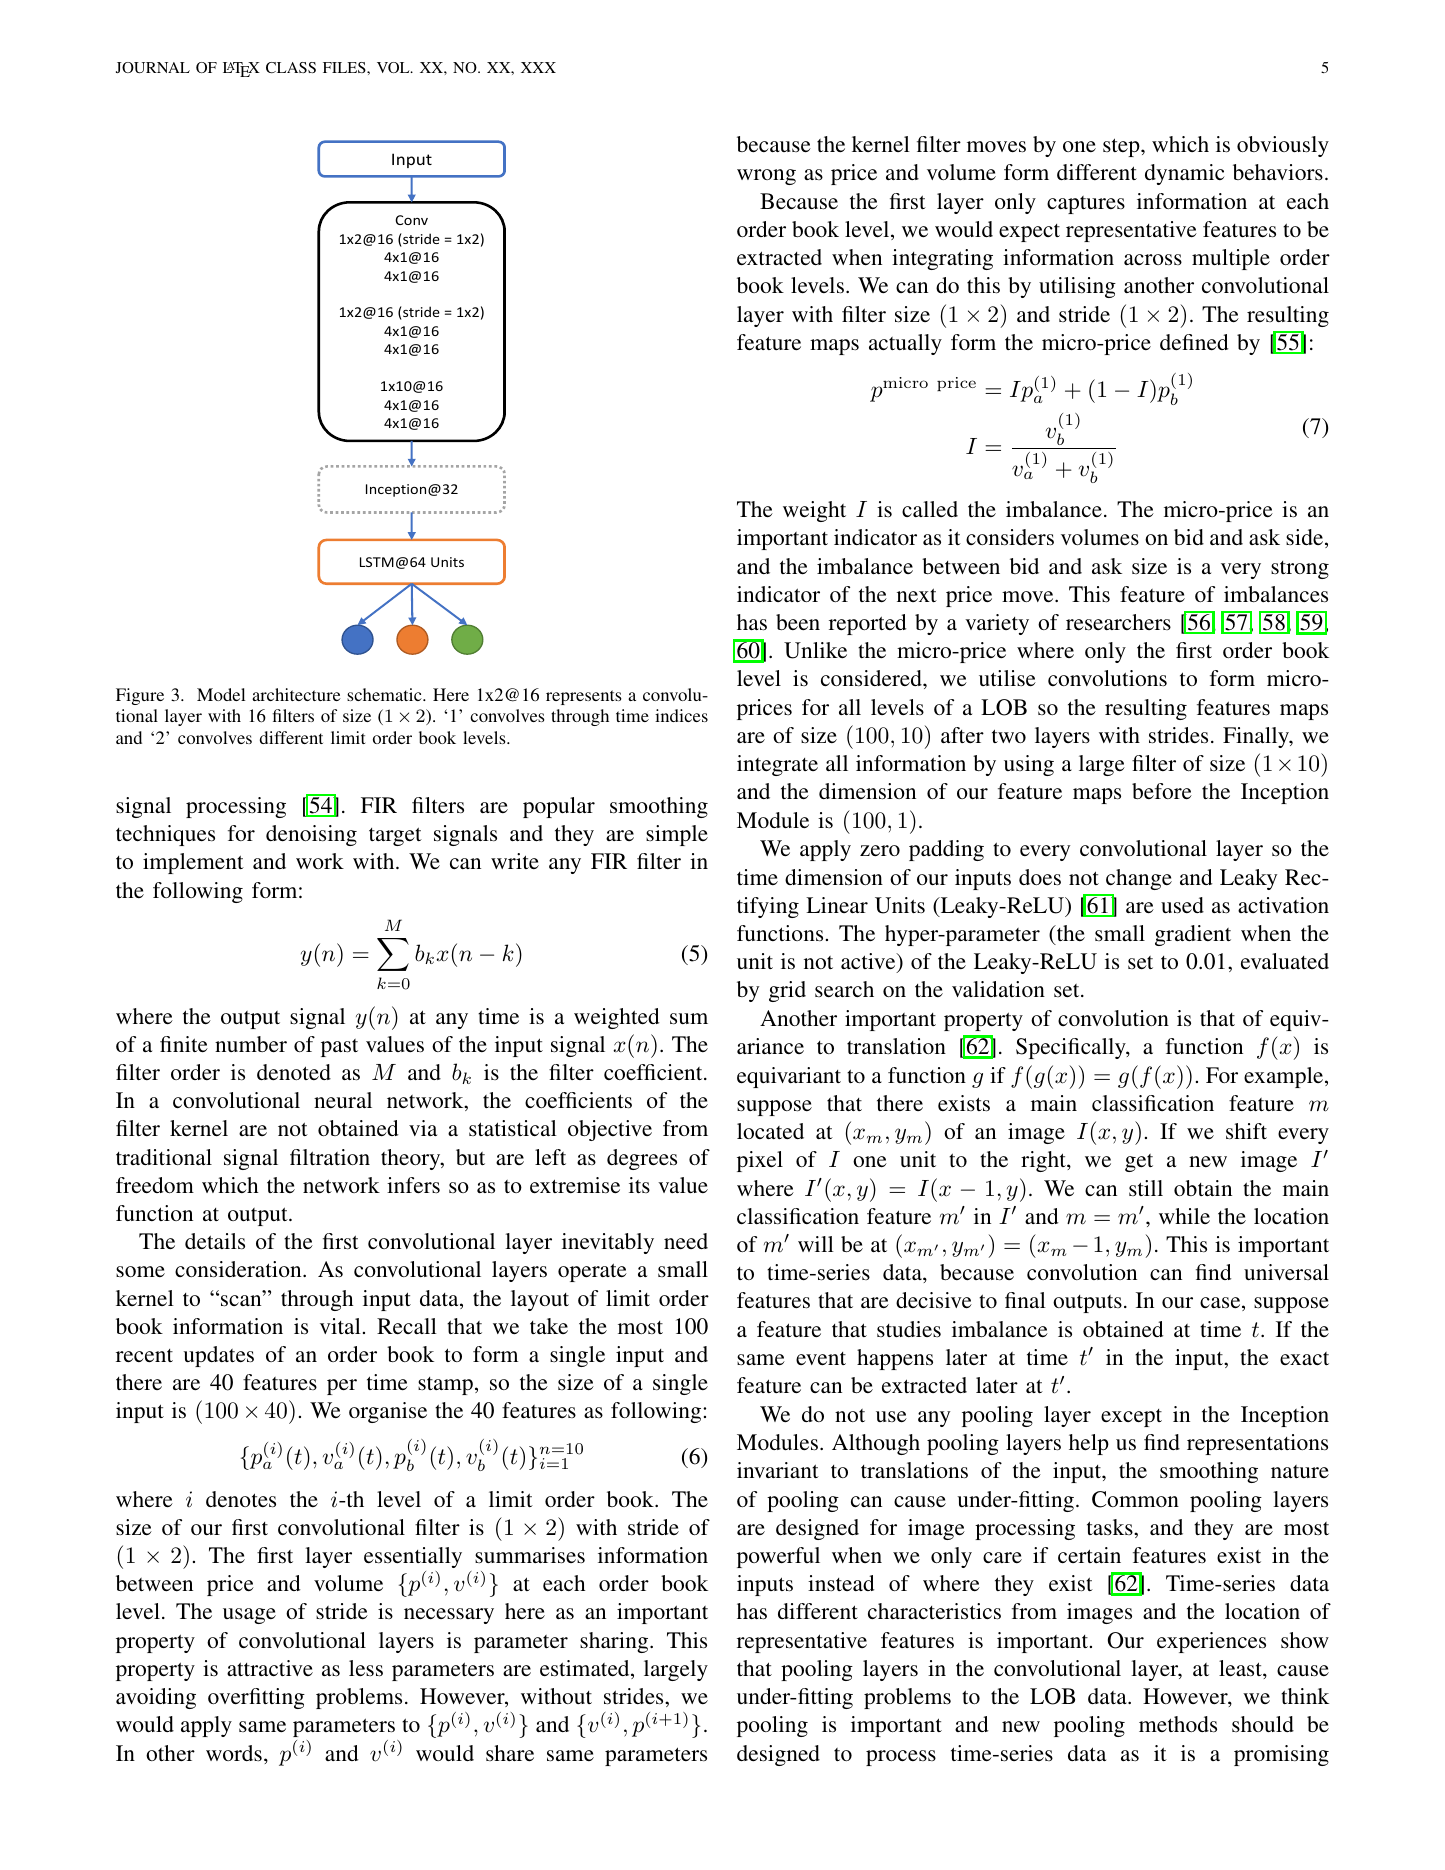
\includegraphics[width=\textwidth,height=0.60\textheight,keepaspectratio]{deeplob_arch_fig3.png}
\source{Zhang, Zohren and Roberts, ``Deep Learning for Limit Order Books'', Figure 3.}
\end{column}
\begin{column}{0.44\textwidth}
\begin{itemize}\tightitems
  \item 输入是 \(100\times40\)：100 次更新、10 档买卖盘价格和数量。
  \item CNN：学习局部队列形状，例如 bid/ask imbalance 和 depth slope。
  \item Inception：同时看不同尺度的短期 order-flow pattern。
  \item LSTM：近似条件分布
  \[
    \mathbb{P}(y_{\tau}=c\mid X_\tau).
  \]
\end{itemize}
\vspace{0.25em}
\begin{block}{一句话}
DeepLOB 好用，是因为它把随机队列过程的局部形状和短期路径依赖放进同一个函数近似器。
\end{block}
\end{column}
\end{columns}
\end{frame}

\begin{frame}[plain]
\contentheader{指标 1：MCC 比准确率更稳}
\begin{columns}[T,totalwidth=\textwidth]
\begin{column}{0.48\textwidth}
\begin{itemize}\tightitems
  \item LOB 标签常常不均衡，很多时候“稳定”类占比高。
  \item accuracy 可能被多数类抬高。
  \item MCC 可以理解为“预测标签和真实标签的相关性”。
  \item 随机预测约为 0，完美预测为 1。
\end{itemize}
\end{column}
\begin{column}{0.48\textwidth}
\begin{block}{混淆矩阵视角}
\[
\text{MCC}=F(\text{全部 true/false positive/negative})
\]
\vspace{0.2em}
它不只看“猜对多少”，还看各类之间怎么错。
\end{block}
\begin{block}{主论文发现}
large-tick 股票在多个 horizon 上更稳定、更容易预测；这说明 score 反映的是模型与市场结构的共同结果。
\end{block}
\end{column}
\end{columns}
\end{frame}

\begin{frame}[plain]
\contentheader{主论文关键图：tick 类别改变结果}
\begin{columns}[T,totalwidth=\textwidth]
\begin{column}{0.54\textwidth}
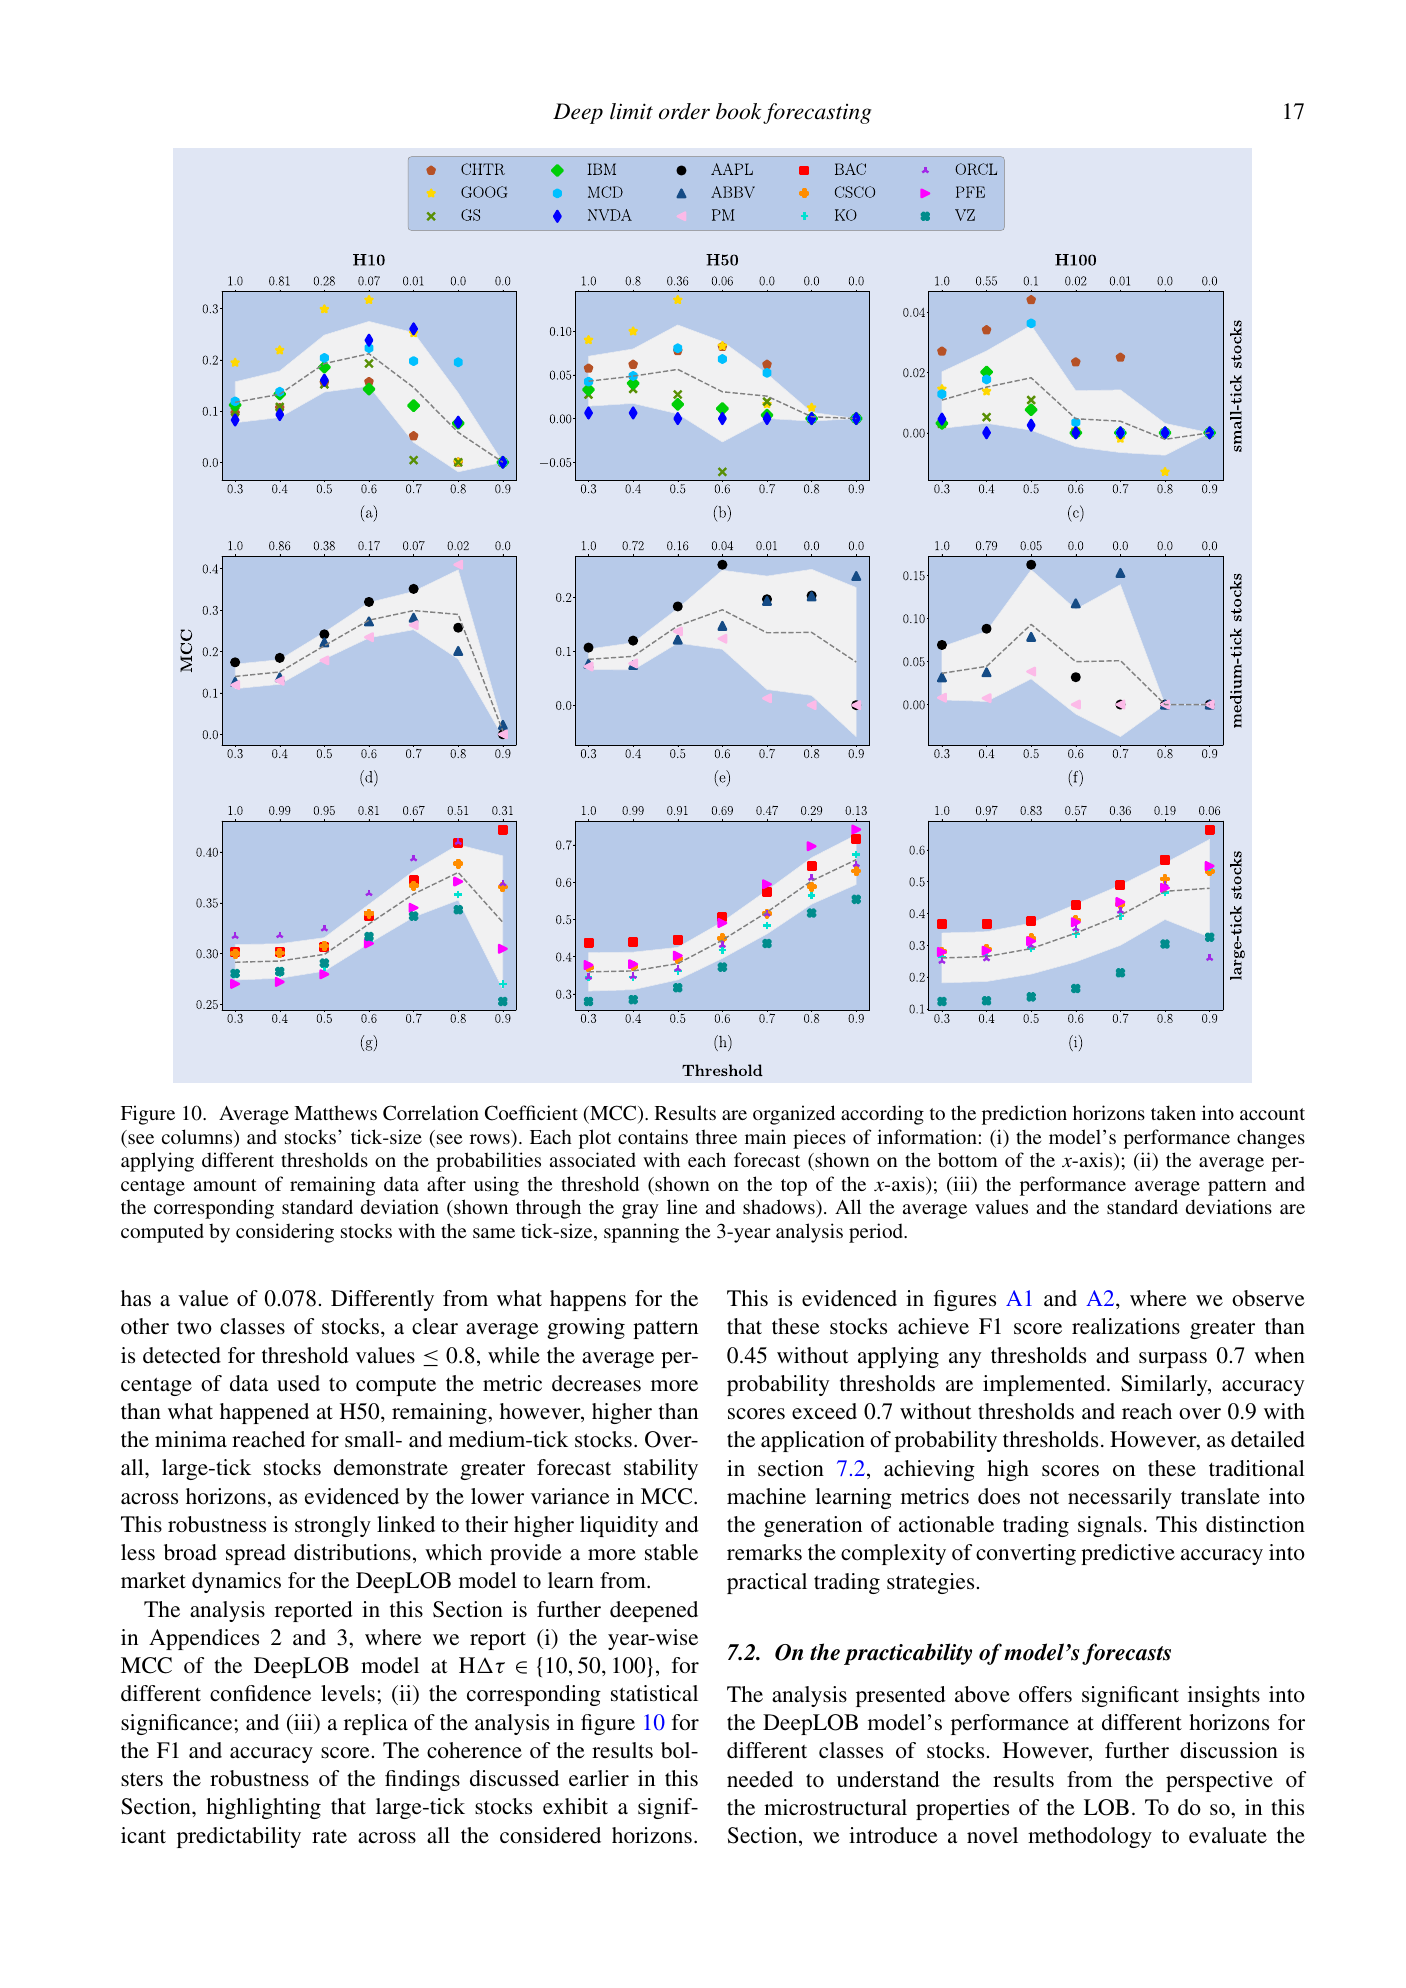
\includegraphics[width=\textwidth,height=0.62\textheight,keepaspectratio]{lobframe_mcc_fig10.png}
\source{Briola et al., Microstructural Guide, Figure 10.}
\end{column}
\begin{column}{0.42\textwidth}
\begin{itemize}\tightitems
  \item 行：small / medium / large tick。
  \item 列：\(H_{10},H_{50},H_{100}\)。
  \item 横轴：只保留更高置信度预测。
  \item 读图结论：模型表现不是单纯由网络决定，而是和股票微观结构强相关。
\end{itemize}
\end{column}
\end{columns}
\end{frame}

\begin{frame}[plain]
\contentheader{指标 2：为什么还需要 \(p_T\)}
\begin{columns}[T,totalwidth=\textwidth]
\begin{column}{0.48\textwidth}
\begin{itemize}\tightitems
  \item F1/MCC 是逐样本指标：每个时间点算一次对错。
  \item 交易是路径问题：需要开仓、持仓、平仓都大致对。
  \item 一个错误如果刚好发生在平仓点，影响比普通点更大。
\end{itemize}
\end{column}
\begin{column}{0.48\textwidth}
\begin{block}{完整交易概率}
\[
P_T=\{\text{模型预测出的完整交易}\}
\]
\[
T_T=\{\text{真实方向对应的完整交易}\}
\]
\[
p_T=\frac{|P_T\cap T_T|}{|P_T\cup T_T|}
\]
\end{block}
\begin{block}{直觉}
\(p_T\) 关心“预测序列能否形成正确交易”，而不只是“单点标签是否正确”。
\end{block}
\end{column}
\end{columns}
\end{frame}

\begin{frame}[plain]
\contentheader{主论文结论：用一句话讲通}
\begin{enumerate}\tightitems
  \item LOB 可预测性不是模型单独决定的，而是由模型、标签、horizon、tick regime 共同决定。
  \item large-tick 股票通常更稳定：价差窄、最优档流动性厚，队列变化更有信息。
  \item 传统分类指标有用，但不够；交易信号还要看时间顺序和完整交易路径。
  \item 这篇文章真正的贡献是：把深度学习预测重新放回市场微观结构里解释。
\end{enumerate}
\vspace{0.35em}
\begin{block}{适合初学者的记法}
先理解市场结构，再评价模型分数；不要反过来只看 leaderboard。
\end{block}
\end{frame}

\section{Other Papers}
\begin{frame}[plain]
\contentheader{其它论文速览（一）：信号与模型}
\begin{columns}[T,totalwidth=\textwidth]
\begin{column}{0.48\textwidth}
\begin{block}{Ait-Sahalia et al.}
\begin{itemize}\tightitems
  \item 高频收益/方向确实存在短寿命可预测性。
  \item 延迟会快速消耗预测价值。
  \item 作用：解释为什么 LOB 信号必须看极短 horizon。
\end{itemize}
\end{block}
\end{column}
\begin{column}{0.48\textwidth}
\begin{block}{DeepLOB}
\begin{itemize}\tightitems
  \item 经典 CNN + Inception + LSTM 结构。
  \item 作用：提供主论文使用的标准模型基线。
  \item 局限：不能单独解决跨市场和交易可用性问题。
\end{itemize}
\end{block}
\end{column}
\end{columns}
\vspace{0.35em}
\centering
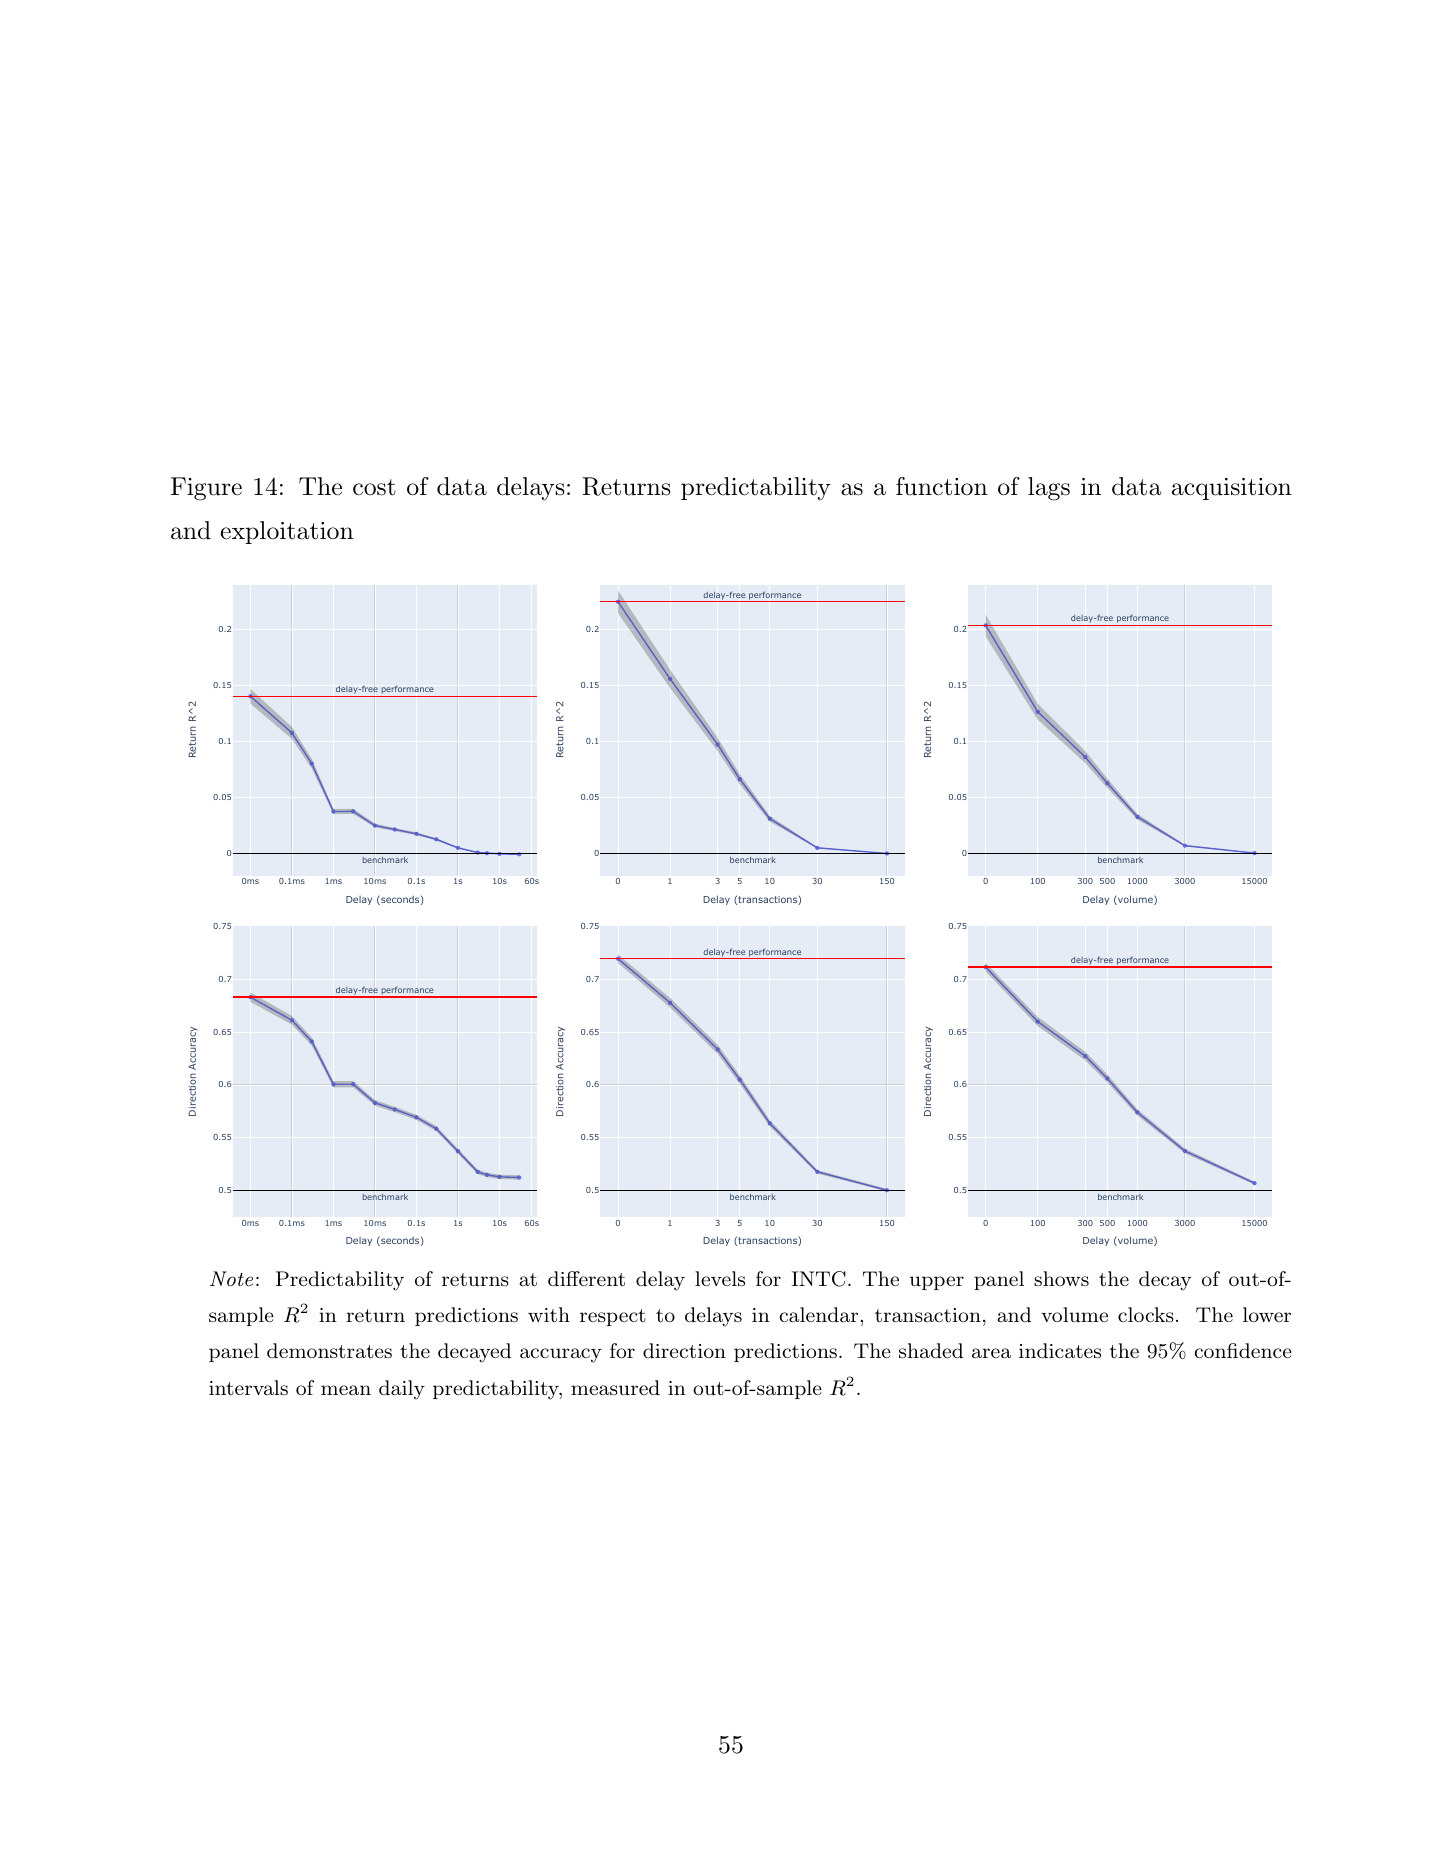
\includegraphics[width=0.68\textwidth,height=0.30\textheight,keepaspectratio]{ait_delay_fig14.png}
\source{Ait-Sahalia, Kalnina and Xiu, Figure 14.}
\end{frame}

\begin{frame}[plain]
\contentheader{其它论文速览（二）：结构与泛化}
\begin{columns}[T,totalwidth=\textwidth]
\begin{column}{0.48\textwidth}
\begin{block}{HLOB}
\begin{itemize}\tightitems
  \item DeepLOB 偏向局部卷积结构。
  \item HLOB 用图结构描述 LOB 变量间依赖。
  \item 作用：说明“市场结构”也可以进入模型设计。
\end{itemize}
\end{block}
\end{column}
\begin{column}{0.48\textwidth}
\begin{block}{Benchmark Study}
\begin{itemize}\tightitems
  \item FI-2010 高分不等于真实市场可迁移。
  \item 模型排序会随数据集和 horizon 变化。
  \item 作用：提醒我们做跨股票、跨市场验证。
\end{itemize}
\end{block}
\end{column}
\end{columns}
\vspace{0.35em}
\centering
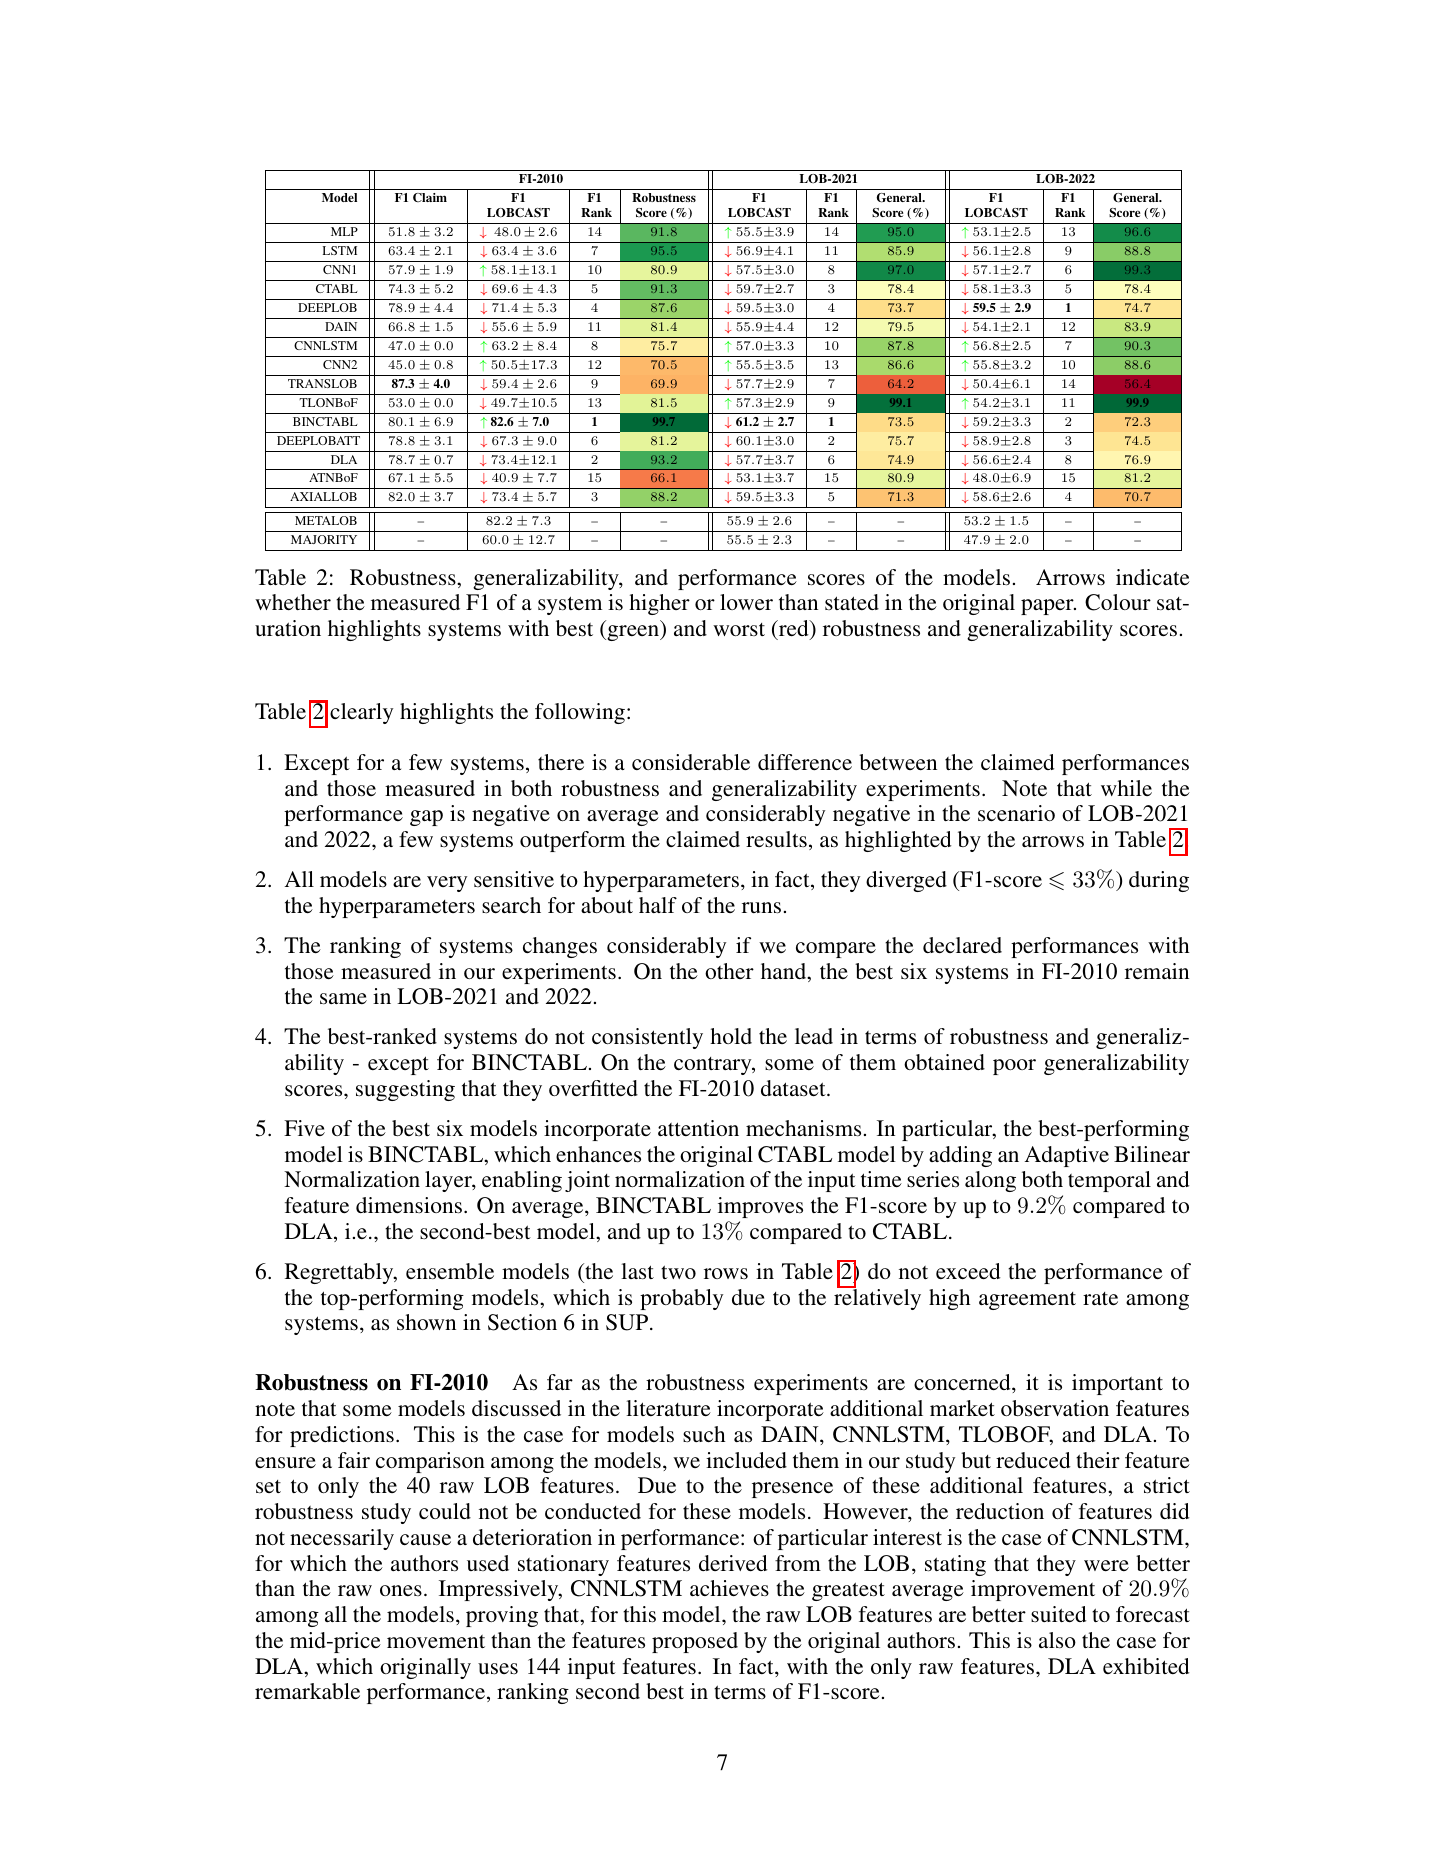
\includegraphics[width=0.76\textwidth,height=0.30\textheight,keepaspectratio]{benchmark_table2.png}
\source{``LOB-Based Deep Learning Models: Benchmark Study'', Table 2.}
\end{frame}

\section{Synthesis}
\begin{frame}[plain]
\contentheader{五篇论文合成一个框架}
\scriptsize
\begin{tabularx}{\textwidth}{>{\bfseries}p{2.2cm}X X}
\toprule
层次 & 要问的问题 & 对应论文 \\
\midrule
信号是否存在 & 极短 horizon 上是否有可预测性？延迟伤害多大？ & Ait-Sahalia et al. \\
输入怎么表示 & LOB 是价格序列，还是买卖盘形状序列？ & DeepLOB \\
市场结构是什么 & tick size、spread、depth 是否改变预测难度？ & Microstructural Guide \\
分数是否可信 & MCC 高是否代表完整交易可用？ & Microstructural Guide \\
模型能否泛化 & 换股票、换市场、换 horizon 后排序是否稳定？ & HLOB / Benchmark Study \\
\bottomrule
\end{tabularx}
\end{frame}

\begin{frame}[plain]
\contentheader{Principle-First Research Logic}
\begin{enumerate}\tightitems
  \item Define the random object: state \(Q_t\), observation \(X_\tau\), and label \(y_\tau\).
  \item Explain the market regime: \(\bar{\sigma}/\theta\), best-queue depth, imbalance, event intensity.
  \item Choose a model bias that matches the object: local convolution, recurrence, graph structure, or point-process intensity.
  \item Evaluate two levels: sample-wise correctness and path-wise tradability.
  \item Test whether the explanation survives across stocks, horizons, and market regimes.
\end{enumerate}
\vspace{0.4em}
\begin{block}{原则}
Model complexity should serve a microstructure explanation; it should not replace one.
\end{block}
\end{frame}

\begin{frame}[plain]
\contentheader{Answers to the Opening Questions}
\begin{enumerate}\tightitems
  \item What is being predicted?\\
  The future direction of the mid-price, usually after a fixed number of LOB updates:
  \[
    y_\tau=g_\theta(m_{\tau+\Delta\tau}-m_\tau).
  \]
  \item Why do tick size, spread, and horizon matter?\\
  They change queue depletion probabilities, class balance, signal lifetime, and transaction-cost meaning.
  \item Why is high accuracy not enough?\\
  A trading signal is a time-ordered path. MCC/F1 count point errors, while \(p_T\) asks whether the predicted path completes the right trade.
\end{enumerate}
\end{frame}

\begin{frame}[plain]
\contentheader{最后的 takeaway}
\begin{enumerate}\tightitems
  \item LOB 预测的核心对象是“订单簿状态序列”，不是单纯价格序列。
  \item LOB 可以看成由订单到达、成交和撤单驱动的随机队列过程。
  \item tick size 是理解可预测性的入口变量，因为它改变队列、价差和标签的尺度。
  \item DeepLOB 是一个好 baseline，但主论文强调的是何时有效、为什么有效。
  \item MCC 比准确率更适合不均衡分类；\(p_T\) 更贴近交易路径。
  \item 真实研究不能只看一个 benchmark 分数。
\end{enumerate}
\vspace{0.45em}
\begin{block}{一句收束}
不要先问“哪个模型最强”；先问“这个市场结构下，什么方向信号在什么 horizon 上可预测，并且能否形成完整交易路径”。
\end{block}
\end{frame}

\begin{frame}[plain]
\contentheader{讨论问题}
\begin{itemize}\tightitems
  \item 如果 MCC 上升但 \(p_T\) 下降，这个模型该怎么用？
  \item 对 small-tick 股票，应优先改标签、改输入表示，还是改模型结构？
  \item 事件时间 horizon 和物理时间 horizon，哪个更适合我们的策略目标？
\end{itemize}
\vspace{0.8em}
\centering
{\Large Q \& A}
\end{frame}

\begin{frame}[plain]
\contentheader{文献与图表来源}
\scriptsize
\begin{itemize}\tightitems
  \item A. Briola, S. Bartolucci, and T. Aste, ``Deep Limit Order Book Forecasting: A Microstructural Guide,'' Quantitative Finance, 2025.
  \item Z. Zhang, S. Zohren, and S. Roberts, ``Deep Learning for Limit Order Books,'' IEEE Transactions on Signal Processing, 2020.
  \item Y. Ait-Sahalia, I. Kalnina, and D. Xiu, ``How and When are High-Frequency Stock Returns Predictable?''
  \item R. Cont and A. de Larrard, ``Price Dynamics in a Markovian Limit Order Market,'' SIAM Journal on Financial Mathematics, 2013.
  \item F. Abergel and A. Jedidi, ``A Mathematical Approach to Order Book Modeling,'' International Journal of Theoretical and Applied Finance, 2013.
  \item E. Bacry, I. Mastromatteo, and J.-F. Muzy, ``Hawkes Processes in Finance,'' Market Microstructure and Liquidity, 2015.
  \item A. Briola et al., ``Information Persistence and Structure in Limit Order Books.''
  \item ``LOB-Based Deep Learning Models: Benchmark Study.''
\end{itemize}
\vspace{0.55em}
{\tiny 注：本 deck 中的论文图表均来自原论文，仅用于内部研究分享；每页图表下方已标注来源。}
\end{frame}

\end{document}
